\chapter{El pronóstico}\label{cap:pron}

La aplicación incluye un pronóstico de hotspots equivalentes a MODIS, diario a 30 días, semanal a 12 semanas y mensual a 12 meses, para cualquier estado o para todo México. El modelo es sencillo a propósito: lo que se pueda explicar y verificar en una página pesa más que una promesa de precisión que los datos no sostienen.

\section{Qué se pronostica}

Sea $S_t$ la serie diaria armonizada de una región (\emph{Todo México} o un estado), con $t=0$ el 1 de noviembre de 2000. Elegimos un \textbf{origen} $T_0$, el último día observado. El pronóstico usa solo datos con $t\le T_0$ y entrega, para cada periodo futuro $P$, un valor puntual $\widehat Y_P$ y un intervalo de $80\,\%$.

\begin{itemize}
  \item \textbf{Diario}: los 30 días siguientes, $P=\{T_0+h\}$, $h=1,\dots,30$.
  \item \textbf{Semanal}: 12 bloques de 7 días consecutivos, $P_w=\{T_0+7(w-1)+1,\dots,T_0+7w\}$.
  \item \textbf{Mensual}: los 12 meses calendario siguientes. El primer mes incluye la parte ya observada hasta $T_0$.
\end{itemize}

\section{Paso 1: climatología de la misma fecha}

Para un día futuro $t$, la climatología es el promedio, sobre los $K$ años anteriores, del nivel diario alrededor de esa misma fecha del calendario:
\begin{align}
  c_t&=\frac{\sum_{k=1}^{K}\lambda^{\,k-1}\,\overline S_{t,k}}{\sum_{k=1}^{K}\lambda^{\,k-1}},&
  \overline S_{t,k}&=\frac{1}{2W+1}\sum_{j=-W}^{W}S_{t_k+j},\label{eq:clim}
\end{align}
donde $t_k$ es el mismo día del calendario $k$ años antes (el 29 de febrero se trata como 28 de febrero). La suma solo incluye los años $k$ cuya ventana completa $[t_k-W,\,t_k+W]$ ya fue observada, es decir, que termina en $T_0$ o antes. Si ningún año cumple, se usa el promedio diario de los últimos 365 días.

Los valores finales son $K=12$, $\lambda=1$ (todos los años pesan igual) y $W=14$ días.

\paragraph{Interpretación.} $c_t$ estima el nivel esperado de la temporada en esa fecha. Con $K=12$ y $2W+1=29$, cada $c_t$ promedia hasta $12\times29=348$ valores diarios. Promediar reduce el ruido, que es grande porque cada día es un conteo pequeño. La ventana $W$ tiene un costo: en el pico de la temporada la serie sube y baja con rapidez, y una ventana ancha suaviza el máximo. Es el compromiso clásico entre sesgo y varianza: ventana chica, más ruido; ventana grande, más sesgo en las cimas.

\section{Paso 2: ajuste de nivel reciente}

La climatología supone un año promedio. Pero hay años de mucho y de poco fuego, y el comportamiento reciente dice algo sobre el resto del año. Medimos qué tanto se desvía lo observado en los últimos $L$ días del promedio esperado:
\begin{align}
  r=\min\!\left\{4,\;\max\!\left\{\tfrac14,\;\frac{\sum_{t=T_0-L+1}^{T_0}S_t+c_0}{\sum_{t=T_0-L+1}^{T_0}c_t+c_0}\right\}\right\},\label{eq:r}
\end{align}
con $L=28$ días y $c_0=5$. En el denominador, la climatología de los días pasados $c_t$ se calcula con la misma regla de la ecuación~\eqref{eq:clim} y solo con datos hasta $T_0$; si se pudo calcular en menos de $80\,\%$ de esos días, se toma $r=1$ (sin ajuste), y si faltan algunos días la suma se reescala proporcionalmente.

\paragraph{Por qué una razón de totales con pseudoconteo.} Es la misma idea del capítulo~\ref{cap:factor}: la razón de totales es más estable que el promedio de razones diarias, y el pseudoconteo $c_0$ evita que un periodo con casi nada de fuego (por ejemplo, octubre) produzca una razón enorme por dividir entre un número muy pequeño. El recorte a $[1/4,\,4]$ evita ajustes extremos. Si $r>1$ el mes pasado estuvo más activo que lo normal; si $r<1$, menos.

\section{Paso 3: el ajuste se apaga con el horizonte}

Aplicar $r$ de forma permanente sería un error: que las últimas cuatro semanas hayan estado activas informa sobre las próximas semanas, pero poco sobre dentro de cinco meses. Por eso se desvanece de forma exponencial con el horizonte $h=t-T_0$:
\begin{align}
  \boxed{\;\widehat s_{T_0+h}=c_{T_0+h}\cdot\exp\!\bigl(\ln r\cdot e^{-h/\vartheta}\bigr)=c_{T_0+h}\cdot r^{\,e^{-h/\vartheta}}\;},\qquad\vartheta=60\text{ días}.\label{eq:pron}
\end{align}

Los dos extremos tienen sentido. Para $h$ pequeño, $e^{-h/\vartheta}\approx1$ y $\widehat s\approx c\cdot r$: se persiste el nivel reciente. Para $h$ grande, $e^{-h/\vartheta}\to0$ y $\widehat s\to c$: se regresa a la climatología.

\paragraph{Lectura estadística.} En logaritmos, $\ln(\widehat s/c)=\ln r\cdot e^{-h/\vartheta}=\ln r\cdot\varphi^{h}$ con $\varphi=e^{-1/\vartheta}\approx0.9835$ por día: es la \emph{función de respuesta} de un proceso autorregresivo AR(1) en las desviaciones logarítmicas respecto a la climatología. La vida media del ajuste, el horizonte en que su efecto se reduce a la mitad, es $\vartheta\ln2\approx41.6$ días.

\begin{table}[H]
\centering
\caption{Peso del ajuste de nivel, $e^{-h/\vartheta}$ con $\vartheta=60$.}\label{tab:peso}
\small
\begin{tabular}{@{}lrrrrrr@{}}
\toprule
Horizonte $h$ (días) & 1 & 7 & 30 & 60 & 120 & 180 \\
\midrule
Peso del ajuste & 0.98 & 0.89 & 0.61 & 0.37 & 0.14 & 0.05 \\
\bottomrule
\end{tabular}
\end{table}

\begin{figure}[H]
\centering
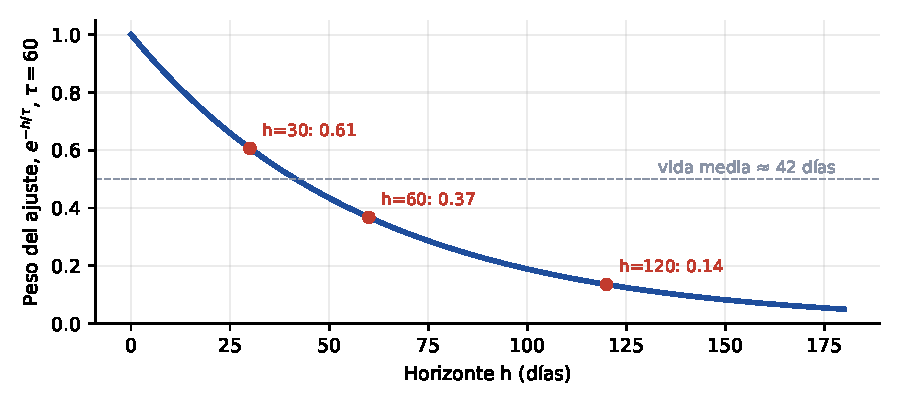
\includegraphics[width=0.82\textwidth]{fig/fig_decaimiento.pdf}
\caption{Peso del ajuste de nivel según el horizonte.}\label{fig:decae}
\end{figure}

\begin{ejemplo}[Cómo se ve con el 2026 de la aplicación]
Con origen el 31 de diciembre de 2025, Todo México sumó $1\,554$ hotspots equivalentes en los últimos 28 días, contra $1\,472$ que daba la climatología: $r\approx1.056$ (con $c_0=5$ casi no cambia). A 30 días el exponente pesa $0.61$ y el ajuste es de $1.056^{0.61}\approx1.033$, o sea $3.3\,\%$ por encima de la climatología. Para mayo (más de 120 días adelante) el exponente pesa menos de $0.14$ y el pronóstico es prácticamente la climatología.
\end{ejemplo}

\section{De la trayectoria diaria a semanas y meses}

El pronóstico de un periodo $P$ es la suma de la parte ya observada y la parte pronosticada:
\begin{align*}
  \widehat Y_P=\underbrace{\sum_{t\in P,\;t\le T_0}S_t}_{\text{observada}}+\underbrace{\sum_{t\in P,\;t>T_0}\widehat s_t}_{\text{pronosticada}}.
\end{align*}
A lo sumo el primer mes calendario tiene parte observada. Al evaluar, el error se mide únicamente en la parte pronosticada, $\widehat Y^{\mathrm{rem}}_P=\sum_{t\in P,\,t>T_0}\widehat s_t$ contra su valor real $Y^{\mathrm{rem}}_P$, para que la parte conocida no regale precisión.

\section{Intervalos de \texorpdfstring{$80\,\%$}{80 \%} con errores del propio modelo}\label{sec:interv}

El intervalo no sale de una distribución supuesta sino de los errores que el modelo \emph{habría cometido} en el pasado.

\paragraph{Error relativo en logaritmos.} Para un origen histórico $T$ y un periodo $P$ con $n_P$ días por pronosticar, definimos
\begin{align*}
  \rho_{T,P}=\ln\frac{Y^{\mathrm{rem}}_{T,P}+\kappa\,n_P}{\widehat Y^{\mathrm{rem}}_{T,P}+\kappa\,n_P},\qquad\kappa=0.5.
\end{align*}
Usamos el cociente y su logaritmo porque el error de un conteo crece con su nivel: equivocarse en 100 hotspots es grave en septiembre y normal en mayo. El pseudoconteo $\kappa\,n_P$ (medio hotspot por día) evita $\ln0$ y el comportamiento errático de los periodos casi vacíos; es la misma estrategia del $c_0$ de la ecuación~\eqref{eq:r}.

\paragraph{Conjunto de errores disponibles.} Se calcula $\rho_{T,P}$ para orígenes semanales desde el 1 de enero de 2003 y para los tres tipos de periodo (día, semana, mes). Para un origen nuevo $T_0$ solo se admiten errores de periodos que \emph{ya terminaron} en $T_0$ o antes (así se evita usar el futuro) y con una estación parecida: la distancia circular en el día del año entre $T$ y $T_0$ debe ser $\le\omega$, con $\omega\in\{45,90,183\}$ días; se toma el menor $\omega$ que deja al menos 40 errores.

\paragraph{Cuantiles y regreso a la escala original.} Sean $q_{10}$ y $q_{90}$ los cuantiles empíricos de $\rho$. El intervalo para la parte pronosticada es
\begin{align*}
  \Bigl[\;\bigl(\widehat Y^{\mathrm{rem}}_P+\kappa n_P\bigr)e^{q_{10}}-\kappa n_P,\;\;\bigl(\widehat Y^{\mathrm{rem}}_P+\kappa n_P\bigr)e^{q_{90}}-\kappa n_P\;\Bigr]_{+},
\end{align*}
donde $[\,\cdot\,]_+$ trunca en 0 el límite inferior; a ambos se les suma la parte observada. El intervalo es multiplicativo y su ancho se adapta a la estación.

\begin{cuidado}[Los intervalos de varios periodos no se suman]
Cada intervalo es de $80\,\%$ para su propio periodo. Sumar los límites de los 12 meses no da un intervalo de $80\,\%$ del total anual: esos errores no son independientes ni tienen el mismo signo. Por eso la aplicación y este documento reportan intervalos por mes, pero no uno del total anual.
\end{cuidado}

\section{Líneas base para comparar}

Un pronóstico solo vale algo frente a otro más simple. Comparamos con:

\begin{enumerate}[label=\arabic*)]
  \item \textbf{Solo climatología}: la ecuación~\eqref{eq:pron} con $r=1$. Aísla la contribución del ajuste de nivel.
  \item \textbf{Mismo periodo del año anterior}: el nivel de la ventana de $\pm14$ días de la misma fecha un año antes ($K=1$, sin ajuste). Es la regla «este año será igual que el pasado».
\end{enumerate}

\section{Elección de los parámetros}

Se exploró una rejilla de $3\times2\times2\times4=48$ combinaciones con $K\in\{4,8,12\}$, $\lambda\in\{1,0.8\}$, $W\in\{7,14\}$ y $\vartheta\in\{0,20,60,150\}$, dejando $L=28$ y $c_0=5$ fijos. El criterio fue el WAPE promedio de los tres niveles (día, semana y mes), promediado con igual peso entre las 33 regiones, con orígenes cada 14 días entre el 1 de enero de 2010 y el 31 de diciembre de 2019. Ganó $K=12$, $\lambda=1$, $W=14$, $\vartheta=60$.

\begin{table}[H]
\centering
\caption{Las cinco mejores combinaciones de la rejilla (WAPE medio entre 33 regiones, \%).}\label{tab:rejilla}
\small
\begin{tabular}{@{}rrrrrrrr@{}}
\toprule
$K$ & $\lambda$ & $W$ & $\vartheta$ & Diario & Semanal & Mensual & Criterio \\
\midrule
\textbf{12} & \textbf{1} & \textbf{14} & \textbf{60} & \textbf{85.0} & \textbf{61.8} & \textbf{51.5} & \textbf{66.1} \\
12 & 0.8 & 14 & 60 & 85.0 & 61.9 & 51.9 & 66.3 \\
12 & 1 & 7 & 60 & 85.5 & 62.5 & 51.6 & 66.5 \\
8 & 0.8 & 14 & 60 & 85.2 & 62.3 & 52.3 & 66.6 \\
12 & 0.8 & 7 & 60 & 85.5 & 62.4 & 51.9 & 66.6

\\
\bottomrule
\end{tabular}
\end{table}

\begin{cuidado}[Dos precisiones]
1) El criterio da el mismo peso a cada región, así que lo domina el desempeño en estados chicos, de errores grandes. 2) $K=12$ y $\lambda=1$ están en el borde de la rejilla: es posible que más años de historia mejoren un poco el pronóstico; no lo exploramos. Además, los periodos objetivo de los últimos orígenes (hasta 12 meses adelante) llegan a 2020, por lo que una fracción pequeña del criterio de ajuste toca ese año.
\end{cuidado}

\section{La prueba hacia atrás}

El modelo se evalúa con \textbf{orígenes semanales del 1 de enero de 2020 al 31 de diciembre de 2025} (314 orígenes). En cada uno se hace el pronóstico con datos hasta ese día, se construyen los intervalos solo con errores ya observables y se compara con lo que ocurrió, para cada región y cada nivel (día, semana, mes). Las métricas son:

\begin{itemize}
  \item \textbf{WAPE} de la parte pronosticada, sumando sobre todos los orígenes y periodos de la región.
  \item \textbf{Sesgo}, $\sum(\widehat Y^{\mathrm{rem}}-Y^{\mathrm{rem}})/\sum Y^{\mathrm{rem}}$.
  \item \textbf{Cobertura} del intervalo de $80\,\%$: proporción de periodos en que lo observado cae dentro del intervalo.
\end{itemize}

\begin{cuidado}[Muestras que se traslapan]
Los pronósticos de orígenes consecutivos se traslapan (la semana siguiente repite casi todo el horizonte), de modo que los errores están correlacionados y el tamaño de muestra efectivo es mucho menor que el número de pares origen--periodo. Por eso no reportamos errores estándar y evitamos dar importancia a diferencias de pocas décimas.
\end{cuidado}

\section{Resultados}

\subsection{Todo México}

\begin{table}[H]
\centering
\caption{Prueba hacia atrás 2020--2025, Todo México. WAPE (\%) del modelo, de la climatología y del año anterior; sesgo del modelo (\%) y cobertura del intervalo de $80\,\%$ (\%).}\label{tab:pron-nac}
\small
\begin{tabular}{@{}lrrrrr@{}}
\toprule
Horizonte & Modelo & Clim. & Año ant. & Sesgo & Cobertura \\
\midrule
Diario (1--30 días) & 30.9 & 31.3 & 37.3 & 2.9 & 85.3 \\
Semanal (1--12 semanas) & 24.8 & 24.3 & 31.3 & 3.6 & 88.8 \\
Mensual (1--12 meses) & 17.9 & 17.5 & 26.1 & 4.9 & 88.7

\\
\bottomrule
\end{tabular}
\end{table}

Lo que dicen los números:

\begin{enumerate}[label=\arabic*)]
  \item El modelo \textbf{supera con claridad} a «igual que el año pasado»: $30.9$ contra $37.3\,\%$ diario, $24.8$ contra $31.3\,\%$ semanal y $17.9$ contra $26.1\,\%$ mensual.
  \item El modelo \textbf{empata con la climatología}: es algo mejor a un día ($30.9$ contra $31.3\,\%$) y algo peor a semanas y meses ($24.8$ contra $24.3\,\%$ y $17.9$ contra $17.5\,\%$). Dadas las muestras que se traslapan, no distinguimos estas diferencias.
  \item El modelo \textbf{sobrestima ligeramente}: entre $+2.9$ y $+4.9\,\%$. No investigamos la causa.
  \item Los intervalos \textbf{cubren más que lo nominal}: entre $85$ y $89\,\%$ para un nivel de $80\,\%$. Son algo anchos.
\end{enumerate}

\begin{figure}[H]
\centering
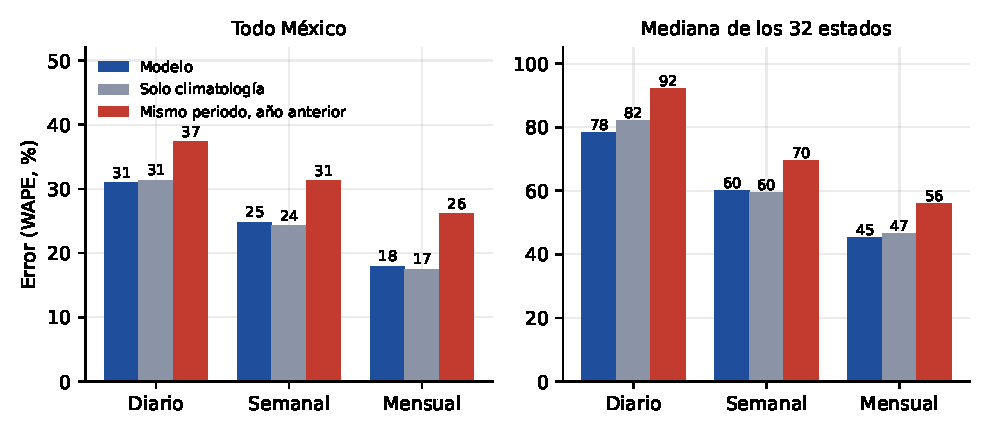
\includegraphics[width=0.98\textwidth]{fig/fig_error_pron.pdf}
\caption{Error de la prueba hacia atrás 2020--2025. Izquierda, Todo México; derecha, mediana de los 32 estados.}\label{fig:error-pron}
\end{figure}

\subsection{Por estado}

\begin{table}[H]
\centering
\caption{Prueba hacia atrás 2020--2025, mediana de los 32 estados. Error mediano (\%) y número de estados (de 32) en que el modelo supera al año anterior y a la climatología.}\label{tab:pron-est}
\small
\begin{tabular}{@{}lrrrrrr@{}}
\toprule
Horizonte & Modelo & Clim. & Año ant. & $<$ año ant. & $<$ clim. & Cobertura \\
\midrule
Diario (1--30 días) & 78.4 & 82.0 & 92.2 & 29 & 22 & 85.2 \\
Semanal (1--12 semanas) & 60.1 & 59.6 & 69.7 & 29 & 26 & 81.7 \\
Mensual (1--12 meses) & 45.3 & 46.6 & 56.1 & 26 & 26 & 82.2

\\
\bottomrule
\end{tabular}
\end{table}

Por estado el error es mucho mayor (mediana de $78\,\%$ diario, $60\,\%$ semanal y $45\,\%$ mensual), sobre todo en estados con pocos hotspots, donde cada día es casi un conteo de cero o uno. El modelo supera al año anterior en 29, 29 y 26 de los 32 estados, y a la climatología en 22, 26 y 26. La cobertura mediana de los intervalos por estado está entre $82$ y $85\,\%$, cercana a lo nominal.

\section{El pronóstico de 2026}

Con origen el 31 de diciembre de 2025, el modelo anticipa para 2026 unos 58.6 mil hotspots equivalentes en México, \crec{}\,\% más que los 52.4 mil de la serie de 2025, con el máximo en mayo (figura~\ref{fig:pron2026}; la tabla~\ref{tab:pron2026} está en el anexo).

\begin{figure}[H]
\centering
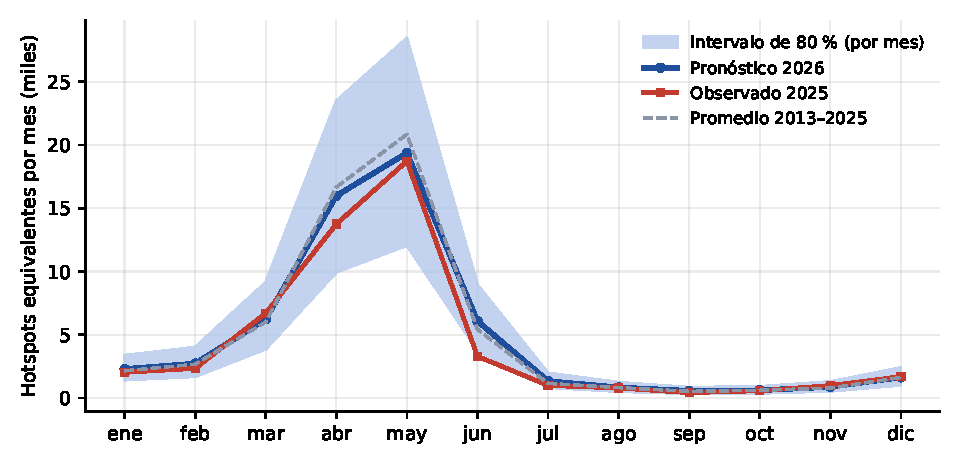
\includegraphics[width=0.95\textwidth]{fig/fig_pron2026.pdf}
\caption{Pronóstico mensual de 2026 para México, con intervalos de $80\,\%$ para cada mes, frente a lo observado en 2025 y al promedio 2013--2025.}\label{fig:pron2026}
\end{figure}

\begin{cuidado}[2026 no se pudo verificar]
Nuestros datos terminan el 31 de diciembre de 2025. No hay forma de comparar este pronóstico con lo que ocurrió en 2026 con la información del proyecto. La prueba hacia atrás dice qué tan bien funcionó el método en 2020--2025; no garantiza nada sobre 2026. En la aplicación se puede escoger un origen anterior y ver el pronóstico contra lo observado.
\end{cuidado}

\begin{ideaclave}[Idea clave del capítulo]
El pronóstico es climatología más un ajuste de nivel que se apaga con el horizonte (ecuación~\eqref{eq:pron}), con intervalos tomados de sus propios errores pasados. A escala nacional empata con la climatología y gana con claridad a repetir el año anterior. Es una línea base estacional con incertidumbre cuantificada, no una predicción de incendios.
\end{ideaclave}
